\section{The \omegamodel\ model}
\label{sec:omega}
\omegamodel\ is a python code developed by Benoit C\^{o}t\'{e} and Christian Ritter\footnote{\url{https://nugrid.github.io/NuPyCEE/}}.
OMEGA stands for 'One-zone Model of the Evolution of Galaxies' and evolves the isotopic content of a galaxy\mycite{cote16a}.
The model is a one-zone model, which means that the entire galaxy is simplified to a single point.
A zero-space-dimensional galaxy model seems unrealistic, but it can be imagined as the mean value for a three-space-dimensional galaxy model.

%Define useful lengths
\newlength{\boxwidth}
\setlength{\boxwidth}{2cm}
\newlength{\boxheight}
\setlength{\boxheight}{1.5cm}
\newlength{\boxdepthx}
\setlength{\boxdepthx}{0.5\boxwidth}
\newlength{\boxdepthy}
\setlength{\boxdepthy}{0.5\boxheight}

%Define useful positions w/short-hand notation
%pos-position, b-bottom, t-top, l-left, r-right, f-front, d-distant
\newcommand\posbfl{(-\boxwidth,-\boxheight)}
\newcommand\posbfr{(\boxwidth,-\boxheight)}
\newcommand\posbdr{(\boxwidth+\boxdepthx,-\boxheight+\boxdepthy)}
\newcommand\posbdl{(-\boxwidth+\boxdepthx,-\boxheight+\boxdepthy)}
\newcommand\postfl{(-\boxwidth,\boxheight)}
\newcommand\postfr{(\boxwidth,\boxheight)}
\newcommand\postdr{(\boxwidth+\boxdepthx,\boxheight+\boxdepthy)}
\newcommand\postdl{(-\boxwidth+\boxdepthx,\boxheight+\boxdepthy)}

\begin{figure}
  \centering
  \begin{tikzpicture}
    %insert galaxy-image in center
    \node (galaxy) at (0.5\boxdepthx,0.5\boxdepthy) {\includegraphics[width=\boxwidth]{galaxy_thumbnail/galaxy.png}};
    %draw bottom plate
    \draw \posbfl -- \posbfr -- \posbdr -- \posbdl -- \posbfl;
    %draw top plate
    \draw \postfl -- \postfr -- \postdr -- \postdl -- \postfl;
    %draw vertical connectors
    \draw \posbfl -- \postfl;
    \draw \posbfr -- \postfr;
    \draw \posbdl -- \postdl;
    \draw \posbdr -- \postdr;
    %add inflow above box
    \draw[thick,->] (0,1.5\boxheight+\boxdepthy) -- (0,1.2\boxheight+\boxdepthy);
    %\draw (-0.5\boxdepthx,2\boxheight) -- (0,2\boxheight-0.5\boxdepthx) -- (0.5\boxdepthx,2\boxheight);
    %\draw (-0.25\boxdepthx,3\boxheight) -- (-0.25\boxdepthx,2\boxheight);
    %\draw (0.25\boxdepthx,3\boxheight) -- (0.25\boxdepthx,2\boxheight);
    \node at (0.6\boxwidth, 1.3\boxheight+\boxdepthy) {\small Primordial gas};
    %add outflow below box
    \draw[thick,->] (0,-1.2\boxheight) -- (0,-1.5\boxheight);
    %\draw (-0.5\boxdepthx,-2\boxheight) -- (0,-2\boxheight-0.5\boxdepthx) -- (0.5\boxdepthx,-2\boxheight);
    %\draw (-0.25\boxdepthx,-1\boxheight) -- (-0.25\boxdepthx,-2\boxheight);
    %\draw (0.25\boxdepthx,-1\boxheight) -- (0.25\boxdepthx,-2\boxheight);
    \node at (0.6\boxwidth, -1.3\boxheight) {\small Enriched gas};
  \end{tikzpicture}
  \caption{\label{tikz:galaxy-iobox}}
\end{figure}


In this work the \omegamodel\ code will be modified with a wrapper in order to explore various parameters related to nucleosynthesis.

\subsection{Process}
\label{sec:omega-process}
The \omegamodel\ model emulates the chemical evolution of a galaxy starting from the initial primordial gas. A simple stellar population is created by integrating the star formation rate over time.
The star formation rate is calculated either by using a constant star formation rate, the Kennicut-Schmidt law\mycitetwo{fuchs09}{and refernces therein}, or by using an input star formation rate and interpolate over those values.

The stellar populations represent a cluster of stars, with a total mass, initial mass distribution, and initial metallicity distribution.
The initial mass distributions are given as one of the standard distributions, Salpeter, Kroupa, Chabrier, or a power-law, all between some minimum and maximum mass limit (see figure \ref{fig:imf}.
The initial metallicity distribution is the relative mass distribution of isotopes heavier than \isotope{Li}{3}{7}, and the metallicity is the mass fraction of all isotopes heavier than \isotope{Li}{3}{7} combined.
\begin{figure}
  \centering
  \includegraphics[width=\textwidth]{img/various_initial_mass_functions.png}
  \caption{ \label{fig:various-imf}
    A simplified visualization of some of the common initial mass functions in the literature.
    \mycitetwo{cappellari12}{and references therein}, \mycite{salpeter55}, \mycite{kroupa01}, \mycite{chabrier03}, \mycite{miller79}. \\
    image-credit: By JohannesBuchner [CC BY-SA 4.0 (\url{https://creativecommons.org/licenses/by-sa/4.0})], from Wikimedia Commons
  }
\end{figure}


Stellar evolution codes calculate the amount of ejected material, for each isotope, for a star with a given initial metallicity and initial mass. These codes are used to create \textbf{yield tables} for certain kind of stars with different initial mass and metallicity.

In the simple stellar population assumed in the galactic chemical evolution model, these yield tables are used to calculate the chemical composition and mass of ejecta from each group of stars. The ejecta are disspersed back into the interstellar medium (gas of the galaxy model) at delay-times appropriate for each group of stellar mass.
E.g. For a given mass-bin the total mass in stars, number, and age of stars, with initial mass in that bin, are calculated using the total mass of the total stellar mass and mass function chosen. By choosing the yield tables closest in initial mass and initial metallicity the total ejecta composition is calculated and added to the interstellar medium at the age where those stars would have gone supernova.
The material that is not ejected is left as remnants and total mass and number of remnants are also added to the simulation at the time these stars would have gone supernova.

In \omegamodel\ the creation and treatment of simple stellar population is done by another python-program called \texttt{Sygma}.

The \omegamodel\ model is a \textit{one-zone} model, meaning that everything inside the box has been enriched from stellar lifecycles. Everything outside the box is untouched since ``it's creation'', and has the same composition as the material inside the box had to start with.
This composition is called the primordial composition (three parts hydrogen, one part helium and trace amounts of lithium and beryllium), and is derived from the big bang nucleosynthesis (see section\ref{sec:bbn}.
Flow of material can determine the chemical evolution of a galaxy. Enriched material can be ejected from the galaxy by supernova feedback, active galactic nucleus, stellar kick or similar, and non-enriched material can flow into the galaxy.
To describe the chemical evolution of a one-zone model one needs to know the total content of the galaxy (or box) and the distribution. In other words, how much of the total mass is stored as each isotope. Material with the same composition as the box is ejected from the box, and material with another composition falls into the box.

\comment{More on outflow/inflow}

\comment{Insert simple figure here}

\subsection{Uncertainty of parameters}
\comment{uncertainty of parameters and summary of article (cote16a)}

Galaxies consist of many different, widely varying, scales for both spatial and temporal resolution.
The galaxies themselves span hydrodynamical evolution on many kpcs and Gyrs, while their stars and supernovae span scales closer to seconds and meters.
The nuclear processes within stars span nanometer and millisecond timescales, even though stars can last for billion years(with short timescale bursts in between).
Neither analytical/numerical models nor simulations cannot cover all these scales at once, that is when subgrid methods are used. Stellar evolution simulations predict the fate and output from the life of a single star based on sinple input parameters and assumptions of the physical processes that governs the evolution. These solutions are then simplified and applied to more complex galaxy simulations.
Output ejecta from stars are ``looked up in a table'' and applied to the nearby interstellar medium.
All these methods and linked applications introduce some uncertainties and assumptions, both physical and numerical, and these uncertainties are inherited through all methods based on applications of these models. In order to probe how the uncertainties of selected parameters manifest through the resulting galaxy evolution, \mycite{cote16a} presents a simple one-zone, closed-box model of galaxy evolution, called \omegamodel.

%use \figwidth for width of image
\begin{figure}
  \centering
  \includegraphics[width=\figwidth]{img/uncertainty_diagram_cote16a_fig1.png}
  \caption[\mycitetwo{cote16a}{fig.1}]{ \label{img:uncertainty-diagram}
    Qualitative visualization of how uncertainties accumulate in galactic chemical evolution models.
    Experimental data on nuclear reaction rates are uncertain to some degree. The change in rate and uncertainty in stellar conditions are not well known.
    The conditions inside a star of a given mass and metallicity come from 1 dimensional hydrodynamical simulations.
    The combined result from nuclear reactions and hydrodynamical simulations give a stellar models.
    The stellar models are applied to a simple stellar population to account for all the billions of stars in galaxy.
    These stellar models are then applied to a large scale hydrodynamical simulation (like \eris), or a semianalytical galaxy model (like \omegamodel).
    All the steps make assumptions and add uncertainty to the grand total uncertainty that is difficult to map in completeness.

    Diagram is taken from \mycitetwo{cote16a}{fig.1}
  }
\end{figure}


\sygma creates the simplified stellar populations (mass function, total mass, lifetime distribution, initial metallicity).
\omegamodel\ combines several stellar populations to emulate a galaxy evolution.

Stellar yields are tables from stellar evolution simulations.
The tables used in \omegamodel are taken from, among other sources,  NuGrid\footnote{NuGrid collaboration: \href{http://www.astro.keele.ac.uk/nugrid/}{Homepage} \href{https://github.com/nugrid}{Github}} and include AGB stars between 1 and 7 \msol, massive stars between 12 and 25 \msol, all with metallicities at $Z = 0.02, 0.01, 0.006, 0.001, 0.0001$. These tables contain many isotopes between hydrogen and bismuth.

The stellar evolution was calculated with MESA\footnote{MESA is a modular, opensource code to evolve single star systems, and can do so from main sequence to white dwarf stage or core collapse stage. See \href{http://mesa.sourceforge.net}{Homepage} for further information}, post-processing was done with MPPNP \mycite{nugrid08mppnp}, the same nuclear reaction rates were used in all calculations, explosive nucleosynthesis was done with semi-analytical models. Yields are complemeted with SN1a yields from \mycite{sn1aivo13}, \mycite{sn1at03}, \mycite{sn1ai99}, \mycite{sn1at86} and population III yields from \mycite{pop3hw10} (other sources are available from the literature, but these are the focus of the chemical evolution of this thesis. Sources for neutron star mergers will be discussed later).

The probability distribution functions for the input parameters are created from values and uncertainties in the literature.
Methodologically there are, for each input parameter, gathered a list of literature values and uncertainties.
The errors are considered gaussian in nature and distributions are created thereafter,
all the distributions are then averaged to a single distribution.
Then a single gaussian is fitted atop the ``average of gaussians from the literature'',
and the median and standard deviation from
the final fit is used as value and uncertainty for the input parameter in question.

%insert images from cote16a to summarize the parameter-method
\setlength{\subfigwidth}{\linewidth}
\begin{figure}
  \centering
  \includegraphics[width=\subfigwidth]{img/parameter_pdfs_cote16a_fig2.png}
  \includegraphics[width=\subfigwidth]{img/parameter_table_cote16a_table7.png}
  \caption{\label{fig:cote16-input-param}
    How the input parameters were determined from multiple sources in the literature. Values and standard deviations averaged to a probaiblity distribution, and then fitted to a single gaussian distribution. Images from \mycitetwo{cote16a}{figure 2 and table 7}.
  }
\end{figure}

\mycite{cote16a} sampled a set calculations, for each parameter in figure \ref{fig:cote16-input-param} a series of 300 calculations were made with a random sampling of the input parameter for the gaussian uncertainty distribution.
A set of 700 calculations were made were all the input parameters were all the input parameters were randomly drawn from their respective gaussian distributions. An additional 300 calculations were made with the final gas-mass and final stellar mass both drawn randomly from their respective gausssian distributions.

Spectroscopic abundance of metals are measured in [X/Y] where X is the metal in question and Y is the reference metal, either plotted against metallicity, [Y/H], or galactic time, Gyr.

The main conclusions are summarized as follows:
\begin{enumerate}
\item{
  The overall uncertainty of spectroscopic metals between 0 and 0.6 dex when plotted against metallicity, but the uncertainty is higher when considered against galactic time.}
\item{
  \begin{itemize}
  \item{Ratio of final mass of gas to final mass of stars affect the uncertianty for early times ([Fe/H] $\lesssim$ -2) since more gas means more hydrogen, while more stars means more iron-production. Since metals are also produced in stars, the ratio does not affect [X/fe] much.}
  \item{Number of type 1a supernovae and their delay time distribution affect the uncertainty of spectroscopic metals at later times([Fe/H] $\gtrsim$ -1.5 $\rightarrow$ t $\gtrsim$ 150Myr), when the delay-time has allowed for type 1a supernovae to occur. Type 1a supernovae add mostly iron to the interstellar medium, while not producing much of metals produced by AGB stars and massive stars. This means that the uncertainty of [X/Fe] will be greatly affected by uncertianties in type 1a supernovae.}
  \item{The high mass slope of the initial mass function, $\alpha$, determines the ratio of massive stars to low-mass stars at all times. Massive stars die quickly and distributed much enriched material into the interstellar medium. Therefor the uncertainty of the slope will always be prevailent in the uncertainty of spectroscopic metals.}
  \item{Uncertainties in the mass ranges of the initial mass function does not affect uncertainties of the spectroscopic abundances much.}
  \end{itemize}
}
\item{
  Uncertainties in the slope of the initial mass function, $\alpha$, and the number of type 1a supernovae affect the uncertainties in the spectroscopic abundances.
  When plotted against metallicity ([Fe/H]) the uncertainty is greatest when the considered metal and the reference metal is not from the same source.
}
\item{
  The characteristics seen from spectroscopic abundance against metallicity is shared regardless of the introduced uncertainties.
  The introduced uncertainties amplify the characterstic shapes, but do not change them. ``Such features are mainly caused by the choice of stellar yields and the type of galaxy considered.''\mycitetwo{cote16a}{p.18}
}
\end{enumerate}

%use \figwidth for width of figure
  \centering
  \includegraphics[width=\figwidth]{img/spectroscopic_uncertainties_cote16a_fig6.png}
  \caption[\mycitetwo{cote16a}{fig.6}]{
    \label{img:spectroscopic-uncertainty}
    Spectroscopic abundance of 16 metals relative to iron, considering uncertainties of all parameters (upper bound, lower bound and high mass slope of initial mass function, stellar and gas mass today, number of type 1a supernovae and the slope of the type 1a supernova delay-time distribution).

    Plots and figures are taken from \mycitetwo{cote16a}{fig.6}
  }

%use \figwidth for width of figure

\begin{figure}
  \centering
  \includegraphics[width=\figwidth]{img/age_uncertainties_cote16a_fig11.png}
  \caption[\mycitetwo{cote16a}{fig.6}]{
    \label{img:age-uncertainty}
    Uncertainty of spectroscopic abundance of 16 metals relative to iron, considering uncertainties of all parameters (upper bound, lower bound and high mass slope of initial mass function, stellar and gas mass today, number of type 1a supernovae and the slope of the type 1a supernova delay-time distribution).

    Uncertainties relative to mean shown as a function of galactic age.

    Plots and figures are taken from \mycitetwo{cote16a}{fig.6}
  }
\end{figure}


\FloatBarrier

\subsection{Relevant parameters}
\label{sec:omega-parameters}
\omegamodel\ has many input parameters, both numerical and physical in nature, to guide the evolution of the galaxy. A physical input parameters are model parameters, while a numerical parameter decides on which calculations to choose from and where to get data. E.g initial gas of galaxy is considered physical, while the boolean switch to turn on neutron star mergers are considered numerical

This section will describe the most relevant ones in order of appearance in the program.

\begin{description}
\item[galaxy]
  This string option chooses predefined parameters to best match a certain galaxy on record.
  The relevant options are:
  \begin{description}
  \item[None] No parameters determined.
  \item[milky\_way\_cte] Set present dark matter mass to $10^{12} \msol$ and present stellar mass to $5\times10^{10} \msol$, and use a constant star formation rate of $1 \frac{\msol}{yr}$
  \item[milky\_way] Set present dark matter mass to $10^{12} \msol$ and present stellar mass to $5\times10^{10} \msol$, and use the star formation rate from \mycite{sfrcmr01}
  \end{description}
\item[in\_out\_control] Boolean switch to turn on or off inflow and outflow.
\item[outflow\_rate] \comment{remove this?} Constant outflow rate in $\frac{\msol}{yr}$. Enriched gas from the interstellar medium is removed from the galaxy.
\item[inflow\_rate] Constant inflow rate in $\frac{\msol}{yr}$. Gas with primordial composition \comment{(reference to BBN?)} flows into the galaxy.
\item[mass\_loading] Fraction of solar masses ejected per solar mass created as star. A different way of calculating outflow based on star formation rate.
\item[imf\_type] Which form to use for the initial mass function\comment{explain this somewhere}. 
\item[alphaimf] Slope of lognormal initial mass function. 
\item[sn1a\_rate] This string option chooses which distribution to calculate the rate of type 1a supernovaefrom.
  Options are powerlaw, gaussian, and exponential distribution.
  \begin{description}
  \item[beta\_pow] Set the power of the power law distribution if 'sn1a\_rate' is "power\_law" 
  \item[gauss\_dtd] Set the mean and standard deviation of the gaussian distribution if 'sn1a\_rate' is "gauss" 
  \item[exp\_dtd] Set the e-folding time of the exponential distribution if 'sn1a\_rate' is "exp"
  \end{description}
\item[dt] Length of first timestep (in yrs)
\item[special\_timesteps] Number of logarithmic timesteps
\item[tend] Final point in time (in yrs)
\item[mgal] Initial mass of gas (if not calculated by other means), defaults to $10^{10} \msol$
\item[transitionmass=8]
  Mass-limit that separates the AGB stars from the massive stars\comment{explain these stars somewhere}.
  Defaults to $8\msol$
\item[nb\_nsm\_per\_m] Set the number of neutron star mergers per solar mass formed as stars.
\item[t\_nsm\_coal] Set the time after which all neutron stars collide/merge
\item[table] path to yield table for AGB and massive stars.
\item[sn1a\_on] Boolean switch that turn on or off the use of type 1a supernovae.
\item[nsm\_dtd\_power] Set the powerlaw distribution of the neutron star merger delay-time distribution \comment{explain this somewhere}.
\item[sn1a\_table] Yield table for type 1a supernovae
\item[ns\_merger\_on] Boolean switch to turn on or off binary neutron star mergers
\item[f\_merger] Fraction of binary systems that eventually merge. All systems are considered binary. This is instead of 'nb\_nsm\_per\_m'
\item[m\_ej\_nsm] solar masses ejected per neutron star merger.
\item[nsmerger\_table] Yield table of binary neutron star mergers
\item[bhns\_merger\_on] Boolean switch to turn on or off black hole neutron star mergers
\item[pop3\_table] Yield tables for population III stars
\item[imf\_bdys\_pop3] The boundaries of the initial mass function of population III stars.
\item[nb\_1a\_per\_m] The number of type 1a supernovae per solar mass formed.
  Used to calculate the number of type 1a supernovae from star formation rate.
\item[popIII\_on] Boolean switch that turn on or off the use of Population III stars
\item[out\_follows\_E\_rate] Adds a time-delay to outflow with mass\_loading such that outflow follows supernova rate.
\item[sfh\_array] Two one-dimensional arrays, time and star formation rate, that \omegamodel will interpolate over in order to find the star formation rate at a given time.
\end{description}
